\documentclass[twoside]{article}
\usepackage[top=1in, bottom=1in, left=0.75in, right=0.75in, columnsep=20pt]{geometry}
\usepackage[framed,numbered,autolinebreaks,useliterate]{mcode}
\usepackage{listings}
\usepackage{graphicx}
\usepackage{tikz}
\usetikzlibrary{arrows}

\usepackage{lipsum} % Package to generate dummy text throughout this template

\usepackage[sc]{mathpazo} % Use the Palatino font
\usepackage[T1]{fontenc} % Use 8-bit encoding that has 256 glyphs
\linespread{1.05} % Line spacing - Palatino needs more space between lines
\usepackage{microtype} % Slightly tweak font spacing for aesthetics

%\usepackage[hmarginratio=1:1,top=32mm,columnsep=20pt]{geometry} % Document margins
\usepackage{multicol} % Used for the two-column layout of the document
\usepackage[hang, small,labelfont=bf,up,textfont=it,up]{caption} % Custom captions under/above floats in tables or figures
\usepackage{booktabs} % Horizontal rules in tables
\usepackage{float} % Required for tables and figures in the multi-column environment - they need to be placed in specific locations with the [H] (e.g. \begin{table}[H])
\usepackage{hyperref} % For hyperlinks in the PDF

\usepackage{lettrine} % The lettrine is the first enlarged letter at the beginning of the text
\usepackage{paralist} % Used for the compactitem environment which makes bullet points with less space between them

\usepackage{abstract} % Allows abstract customization
\renewcommand{\abstractnamefont}{\normalfont\bfseries} % Set the "Abstract" text to bold
\renewcommand{\abstracttextfont}{\normalfont\small\itshape} % Set the abstract itself to small italic text

\usepackage{titlesec} % Allows customization of titles
\renewcommand\thesection{\Roman{section}} % Roman numerals for the sections
\renewcommand\thesubsection{\Roman{subsection}} % Roman numerals for subsections
\titleformat{\section}[block]{\large\scshape\centering}{\thesection.}{1em}{} % Change the look of the section titles
\titleformat{\subsection}[block]{\large}{\thesubsection.}{1em}{} % Change the look of the section titles

\usepackage{fancyhdr} % Headers and footers
\pagestyle{fancy} % All pages have headers and footers
\fancyhead{} % Blank out the default header
\fancyfoot{} % Blank out the default footer
\fancyhead[C]{EECS C149 : DESIGN OF CYBER-PHYSICAL SYSTEMS \hfill October 8, 2014} % Custom header text
\fancyfoot[RO,LE]{\thepage} % Custom footer text

%----------------------------------------------------------------------------------------
%	TITLE SECTION
%----------------------------------------------------------------------------------------

\title{\vspace{-15mm}\fontsize{24pt}{10pt}\selectfont\textbf{I Robot Hill Climb in C}} % Article title

\author{
\large
\textsc{Aaron Feldman, Antonio Rohit}\\[2mm] % Your name
\normalsize University of California, Berkeley \\ % Your institution
\vspace{-5mm}
}
\date{}

%----------------------------------------------------------------------------------------

\begin{document}

\maketitle % Insert title

\thispagestyle{fancy} % All pages have headers and footers

%----------------------------------------------------------------------------------------
%	ABSTRACT
%----------------------------------------------------------------------------------------

\begin{abstract}

\noindent This lab builds on programming cyber-physical systems, specifically feedback-control. Using Microsoft Visual Studio Express, we implemented a state machine in C that instructs the iRobot Create to navigate to the top of an incline while avoiding cliffs and obstacles in a simulated environment. Then using C \& C++ Development Tools for NI Linux Real-Time, Eclipse Edition, we implemented a state machine in C on myRIO that instructs the iRobot Create to navigate to the top of an incline while avoiding cliffs and obstacles in a real physical environment.

\end{abstract}

%----------------------------------------------------------------------------------------
%	ARTICLE CONTENTS
%----------------------------------------------------------------------------------------

\vspace{-3mm}
\begin{center}
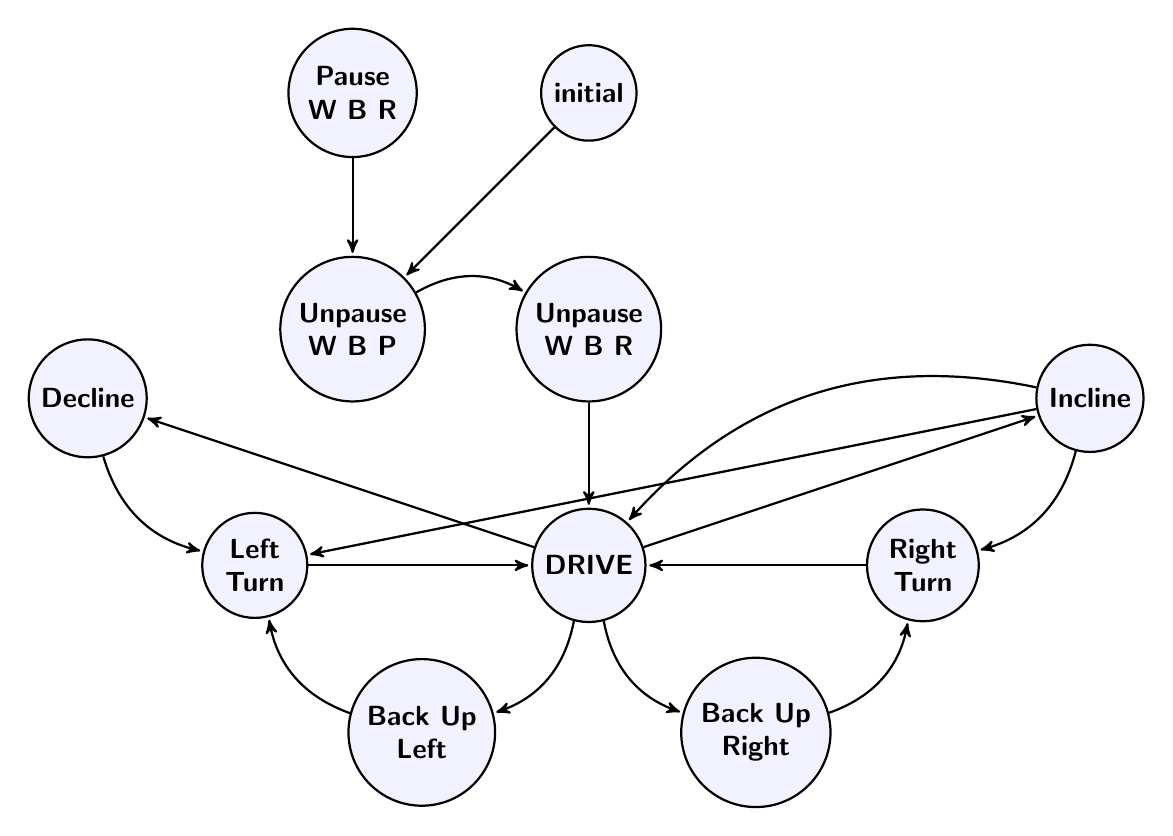
\begin{tikzpicture}[->,>=stealth',shorten >=1pt,auto,node distance=3cm,
  thick,main node/.style={circle,fill=blue!5,draw,font=\sffamily\bfseries}]
  \node[main node, align=center] (1) {initial};
  \node[main node, align=center] (2) [left of=1]{Pause\\ W B R};
  \node[main node, align=center] (3) [below of=1]{Unpause\\ W B R};
   \node[main node, align=center] (4) [left of=3]{Unpause\\ W B P};
  \node[main node, align=center] (5) [below  of=3]{DRIVE};
  \node[main node, align=center] (6) [below left of=5]{Back Up\\ Left};
   \node[main node, align=center] (7) [below right of=5]{Back Up\\ Right};
  \node[main node, align=center] (8) [above right of=7]{Right\\ Turn};
  \node[main node, align=center] (9) [above right of=8]{Incline};
   \node[main node, align=center] (10) [above left of=6]{Left\\ Turn};
  \node[main node, align=center] (11) [above left of=10]{Decline};

  \path[every node/.style={font=\sffamily\small}]
  
(1) edge [] node [left] {} (4)
(2) edge [] node [left] {} (4)     
(3) edge [] node [left] {} (5)  
(4) edge [bend left] node [left] {} (3) 
(5) edge [bend left] node [left] {} (6)
	  edge [bend right] node [left] {} (7) 
	  edge [] node [left] {} (9) 
	  edge [] node [left] {} (11) 
(6) edge [bend left] node [left] {} (10)
(7) edge [bend right] node [left] {} (8)
(8) edge [] node [left] {} (5)
(9) edge [bend left] node [left] {} (8)
      edge [bend right] node [left] {} (5)
      edge [] node [left] {} (10)
(10) edge [] node [left] {} (5)
(11) edge [bend right] node [left] {} (10)


 ;
\end{tikzpicture}
\end{center}


%\begin{multicols}{2} % Two-column layout throughout the main article text

\section{Hill Climb in Simulation}
For the hill climb simulation we programmed the virtual robot in Microsoft Visual Studio 2013a. It was in the simulator that we designed the states for the robot to follow. The states can be seen in the image above. I did however exclude the logic and paths to the pause state for readability.\\

\noindent The code for the hill climb was broken down into a few separate areas: an area for declarations, an area for calculations and resets, an area for pause state transitions, an area for run state transitions, and an area for state actions. Most of the logic we programmed was in the drive state. This allowed us to program for cliffs and obstacles and to transition from drive when such things were encountered and to transition back to drive so that the robot would be ready when such conditions occurred again.\\

\vspace{5mm}
\begin{lstlisting}[mathescape, frame=single]
case DRIVE:
		if (downclineState && abs(accel.y) <= 0.08 && abs(accel.z) >= 0.99 && abs(accel.x) <= 0.08 && (abs(netDistance - distanceAtDownclineStart) >= downclineDistanceThreshold)) {
			state = UNPAUSE_WAIT_BUTTON_PRESS;
		} else if (sensors.cliffFrontLeft || sensors.cliffFrontRight) {
			//state = DOWNCLINE;
			state = BACKUP_RIGHT;
			downclineState = true;
			distanceAtDownclineStart = netDistance;
		} else if (sensors.cliffLeft) {
			turnAmount = 25;
			state = RIGHT_TURN;
		} else if (sensors.cliffRight) {
			turnAmount = 25;
			state = LEFT_TURN;
		} else if (((((accel.x > xAccelInclineThreshold || accel.x < -xAccelInclineThreshold) || (accel.y > yAccelInclineThreshold || accel.y < -yAccelInclineThreshold) ) && accel.z < zAccelInclineThreshold ) && !first_incline_set) && !(sensors.bumps_wheelDrops.bumpLeft || sensors.bumps_wheelDrops.bumpRight || downclineState)) {
			state = UPINCLINE;
		} else if (sensors.bumps_wheelDrops.bumpLeft) {
            state = BACKUP_RIGHT;
			turnAmount = bumpTurnAmount;
            distanceAtManeuverStart = netDistance;
        } else if (sensors.bumps_wheelDrops.bumpRight) {
            state = BACKUP_LEFT;
			turnAmount = bumpTurnAmount;
            distanceAtManeuverStart = netDistance;
        } else {
            if (((netAngle - desiredAngle) < -5) && (abs(netDistance - distanceAtManeuverStart) >= 150)){
                state = LEFT_TURN;
				turnAmount = abs(netAngle - desiredAngle);
            }
            if (((netAngle - desiredAngle) > 5) && (abs(netDistance - distanceAtManeuverStart) >= 150)){
                state = RIGHT_TURN;
				turnAmount = abs(netAngle - desiredAngle);
            }
        }
\end{lstlisting}

\noindent We used feedback from the accelerometer to differentiate between states like drive and incline. We decided to go for the simple approach and try isolating values for the x, y, z accelerometers to determine if the iRobot was on an incline. We found for the simulation this worked rather well with certain thresholds set. 

\vspace{-3mm}
\begin{lstlisting}[mathescape, frame=single]
static double zAccelInclineThreshold = 1;
static double yAccelInclineThreshold = 0.1;
static double xAccelInclineThreshold = 0.1;
\end{lstlisting}

\noindent Now then that we knew we were on an incline, we needed to adjust to point directly up the incline. To do this we first we stopped our forward motion to get a more accurate reading on the accelerometers. Then we wanted to detect if we're pointing upward or downward on the incline. If we're pointing downward, first thing we do is turn around 180 degrees to point up the incline. The state then will loop and we then set the initial incline y accelerometer reading. We then turn either right or left depending on if the original incline by 3 degrees at a time, until it reaches the opposite sign. This then we set for our desired angle and we transition to the drive state. From there, if we continue to be on an incline, we recheck our incline every 500mm. We decided to use a low pass averaging filter. However we felt it was unecessary as this part of our algorithm seemed to be working pretty robustly before we introduced the filtering.

\vspace{3mm}
\begin{lstlisting}[mathescape, frame=single]
// lets filter the accelerometer
    medianX = (1 - FILTER_WEIGHT) * medianX + (FILTER_WEIGHT) * accel.x;
    medianY = (1 - FILTER_WEIGHT) * medianY + (FILTER_WEIGHT) * accel.y;
    medianZ = (1 - FILTER_WEIGHT) * medianZ + (FILTER_WEIGHT) * accel.z;
\end{lstlisting}

\vspace{3mm}
\begin{lstlisting}[mathescape, frame=single]
case UPINCLINE: 
		if (accel.x < -0.15) {
			desiredAngle = netAngle + 180;
			turnAmount = 180;
			state = RIGHT_TURN;
		} else if (incline_start_angle < 0 && accel.y < 0) {
			turnAmount = 1;
			state = RIGHT_TURN;
		} else if ((incline_start_angle > 0 && accel.y > 0)) {
			turnAmount = 1;
			state = LEFT_TURN;
		} else {
			first_incline_set = true;
			desiredAngle = netAngle;
			state = DRIVE;
		}
\end{lstlisting}

\noindent Initial testing on CyberSim allowed us to catch many errors quickly and to calibrate many of our thresholds, especially those for detecting inclines. We chose to keep multiple drive speeds, faster for flat, slower for incline, as this allowed us to pass the CyberSim simulations consistently. Going slower on inclines allowed in the simulation for more accurate accelerometer readings and also kept us from going over the edge.\\

\begin{center}
\includegraphics*[width = 15cm]{FIG1.png}\\
Figure 1: myRIO Board Connected to Speaker
\end{center}

%------------------------------------------------

\section{Hill Climb on iRobot}

We found right away that the simulator was quite different from the real world implementation. When we first uploaded our code the the iRobot, it ran in circles. We found out that (some) of the iRobots have the wheels wired opposite. So when you tell the machine to turn right, it turns left and vice versa. So we reversed the wheel direction in our code. Then to trouble shoot we decided to log the states into a file on the iRobot. To do that we used the code below. This allowed us to diagnose and troubleshoot the issues we had with the machine much more efficently and accurately.

\vspace{6mm}
\begin{lstlisting}[mathescape, frame=single]
FILE *fp = fopen("statehistory.txt", "a");
fprintf(fp, "instrument readings");
fclose (fp);
\end{lstlisting}

One of the issues we had with the physical machine was that its accelerometer readings were much more sporadic. This led us to adjusting the thresholds for the accelerometer for the incline settings for better performance. I also tried making a queue of accelerometer measurements and taking a median of the values to throw away outliers. This however, while great in principal, didn't seem to work on the machine, as it slowed the acquisition of the incline state down a bit. Perhaps this would be a good technique to retry in the future when there is more time to test.

\vspace{-3mm}
\begin{lstlisting}[mathescape, frame=single]
static double zAccelInclineThreshold = 0.97;
static double yAccelInclineThreshold = 0.14;
static double xAccelInclineThreshold = 0.14;
\end{lstlisting}

\noindent We also had to increase the incline drive speed, as the iRobot would often get stuck at the beginning of the ramp incline. With those set, then we had to adjust the settings for when we detect the cliff at the end, so the iRobot would reverse for a short distance, or we found that it would often drop a wheel off the side while turning around. We found that we had to include some "corrections" in our code for the physical iRobot in comparision to the simulation. For example we uncorrected an over correction for the angle up an incline. And we also had to adjust from turning around 180 degrees to 170 degrees as we found that is what actually turned the machine around for reverse downward the ramp.

\vspace{-3mm}
\begin{lstlisting}[mathescape, frame=single]
 else if (inclineCorrection){
            inclineCorrection = false;
            turnAmount = 5;
            if (incline_start_angle < 0) {
                state = LEFT_TURN;
            }
            else {
                state = RIGHT_TURN;
            }
        }
\end{lstlisting}

%------------------------------------------------

\section{Feedback}

We found this lab to be a lot of work. We spent not only our lab time, but much of Friday, Saturday, Monday, and Wednesday on this lab to get everything correct. One thing we learned is to try and find a good trouble shooting tool. This for us on this project was logging states and sensor readings on the iRobot. Beyond that, I would recommend in the future that maybe this lab be paced out to be over two weeks. I think this would relieve much of the pressure on students, and would allow more time for experimentation with the iRobot. I have a few ideas that I believe would lead to a better implementation but unfortunately don't have the time to try them out. And it's the trying it out that in the end leads to learning.

%----------------------------------------------------------------------------------------
\newpage
\noindent \textbf{irobotNavigationStatechart.c}
\vspace{-3mm}
\begin{lstlisting}[mathescape, frame=single]
#include "irobotNavigationStatechart.h"
#include <math.h>
#include <stdlib.h>
#include <stdio.h>

/// Program States
typedef enum{
    INITIAL = 0,                        ///< Initial state
    PAUSE_WAIT_BUTTON_RELEASE,          ///< Paused; pause button pressed down, wait until released before detecting next press
    UNPAUSE_WAIT_BUTTON_PRESS,          ///< Paused; wait for pause button to be pressed
    UNPAUSE_WAIT_BUTTON_RELEASE,        ///< Paused; pause button pressed down, wait until released before returning to previous state
    DRIVE,                              ///< Drive straight
    TURN,                               ///< Turn
    RIGHT_TURN,                         ///< Turn right
    LEFT_TURN,                          ///< Turn left
    BACKUP_RIGHT,						///< Backup followed by a right
    BACKUP_LEFT,						///< Backup followed by a left	
    INCLINE,							///< Sets variables to go up hill	
    DECLINE								///< Begin the process going down the hill
} robotState_t;


#define DEG_PER_RAD            (180.0 / M_PI)        ///< degrees per radian
#define RAD_PER_DEG            (M_PI / 180.0)        ///< radians per degree
#define ANGLE_TOLERANCE            (0.01)                // What we can hope is a safe tolerance when dealing with the angle measured by the robot

extern FILE *fp;						///< Pointer to statehistory text file used to log errors. Definition in target/myrio/main.c

void irobotNavigationStatechart(
    const int32_t                 	netDistance,
    const int32_t                 	netAngle,
    const irobotSensorGroup6_t    	sensors,
    const accelerometer_t         	accel,
    const bool                    	isSimulator,
    int16_t * const             	pRightWheelSpeed,
    int16_t * const             	pLeftWheelSpeed
    ){
    // local state
    static robotState_t         	state = INITIAL;                	// Initial state
    static robotState_t            	unpausedState = DRIVE;            	// state history for pause region
    static int32_t                	distanceAtManeuverStart = 0;    	// distance robot had travelled when a maneuver begins, in mm
    static int32_t                	angleAtManeuverStart = 0;        	// angle through which the robot had turned when a maneuver begins, in deg

    // outputs
    int16_t                        leftWheelSpeed = 0;                	// speed of the left wheel, in mm/s
    int16_t                        rightWheelSpeed = 0;            		// speed of the right wheel, in mm/s

    //*****************************************************
    // state data - process inputs                        *
    //*****************************************************
    static int32_t turnAmount;
    static bool first_incline;
    static bool declineState;
    //static bool second_incline;
    static double incline_start_angle;									// y.accel at which we start the incline
    static int32_t desiredAngle;										// trajectory we want to follow
    static bool first_incline_set;										// indicate that we are on the incline
    static int32_t driveSpeed = 200;									// variable holds the speed for the iRobot in drive
    static int32_t bumpTurnAmount = 15;									// deg to turn the robot on a bump or a cliff	
    static int32_t turnSpeed = 50;										// speed to turn at
    static int32_t backUpDistance = 20;									// how far to back up
    static int32_t inclineRecalcDistance = 500;							// after how many mm do you want to recheck trajectory
    static int32_t distanceAtDECLINEStart;								// distance when the edge of the cliff was seen
    static int32_t DECLINEDistanceThreshold = 2000;						// since there is a plateau at the top of the incline, need a thresh after which we want to stopped
    static double zAccInclThresh = 0.96;								// z acc thresh for incline/flat
    static double xAccInclThresh = 0.1;									// x acc thresh for incline/decline/flat
    static double yAccInclThresh = 0.1;									// y acc thresh for incline/decline/flat

	// Let's reset incline values after a certain distance so it can recalc or do multiple inclines
    if ((abs(netDistance - distanceAtManeuverStart) >= inclineRecalcDistance)) {
        first_incline = false;
        first_incline_set = false;
        distanceAtManeuverStart = netDistance;
        driveSpeed = 200;
    }


    //*****************************************************
    // state transition - pause region (highest priority) *
    //*****************************************************
    if (state == INITIAL
        || state == PAUSE_WAIT_BUTTON_RELEASE
        || state == UNPAUSE_WAIT_BUTTON_PRESS
        || state == UNPAUSE_WAIT_BUTTON_RELEASE
        || sensors.buttons.play                // pause button
        ){
        switch (state){
        case INITIAL:
            // set state data that may change between simulation and real-world
            if (isSimulator){
            }
            else{
            }
            state = UNPAUSE_WAIT_BUTTON_PRESS; // place into pause state
            break;
        case PAUSE_WAIT_BUTTON_RELEASE:
            // remain in this state until released before detecting next press
            if (!sensors.buttons.play){
                state = UNPAUSE_WAIT_BUTTON_PRESS;
            }
            break;
        case UNPAUSE_WAIT_BUTTON_RELEASE:
            // user pressed 'pause' button to return to previous state
            if (!sensors.buttons.play){
                state = unpausedState;
            }
            break;
        case UNPAUSE_WAIT_BUTTON_PRESS:
            // remain in this state until user presses 'pause' button
            if (sensors.buttons.play){
                state = UNPAUSE_WAIT_BUTTON_RELEASE;
            }
            break;
        default:
            // must be in run region, and pause button has been pressed
            unpausedState = state;
            state = PAUSE_WAIT_BUTTON_RELEASE;
            break;
        }
    }

    /*****************************************************
     * THIS SWITCH STATEMENT HANDLES STATE TRANSITIONS   *
     *****************************************************/
    switch (state) {

    /* Drive is the main state in which the robot runs. This state needs to be sensitive to a variety of events
     * 1. THE END OF THE CHALLENGE (Stop)
     * 2. THE CLIFF AT THE TOP OF THE INCLINE (Detect, Backup, and Turn 180)
     * 3. THE EDGES OF THE INCLINE (Avoid like you would a bump)
     * 4. THE INCLINE ITSELF (Go directly up it)
     * 5. OBSTACLES (Avoid the obstacle and then follow original course)
     *
     */
    case DRIVE:
	// This part of DRIVE handles the end of the challenge - we are on the decline, and the x acceleration and z acceleration indicates we are on flat
	// ground. Also, the distance driven away from the cliff (and off the plateau) needs to have crossed a threshold. 
		if (declineState && abs(medianY) <= 0.08 && abs(medianZ) >= 0.99 && abs(medianX) <= 0.08 && (abs(netDistance - distanceAtDownclineStart) >= downclineDistanceThreshold)) {
            state = UNPAUSE_WAIT_BUTTON_PRESS;
            fprintf(fp, "state: 1 UNPAUSE_WAIT_BUTTON_PRESS, accel.x: %+1.3f, accel.y: %+1.3f, accel.z: %+1.3f      leftBump: %d, rightBump: %d, leftCliff: %d, rightCliff: %d, frontLeftCliff: %d, frontRightCliff: %d \n", accel.x, accel.y, accel.z, sensors.bumps_wheelDrops.bumpLeft, sensors.bumps_wheelDrops.bumpRight, sensors.cliffLeft, sensors.cliffRight, sensors.cliffFrontLeft, sensors.cliffFrontRight);
        }
        // the front cliff sensors indicate the cliff at the top of the hill
		else if ((sensors.cliffFrontLeft || sensors.cliffFrontRight) && !declineState && !onIncline) {
            state = DECLINE;
            declineState = true;
            distanceAtDownclineStart = netDistance;
            fprintf(fp, "state: 2 DECLINE, accel.x: %+1.3f, accel.y: %+1.3f, accel.z: %+1.3f      leftBump: %d, rightBump: %d, leftCliff: %d, rightCliff: %d, frontLeftCliff: %d, frontRightCliff: %d \n", accel.x, accel.y, accel.z, sensors.bumps_wheelDrops.bumpLeft, sensors.bumps_wheelDrops.bumpRight, sensors.cliffLeft, sensors.cliffRight, sensors.cliffFrontLeft, sensors.cliffFrontRight);

        }
		// The edge of incline is detected - treat this like a bump
        else if (sensors.cliffLeft) {
            turnAmount = 25;
            state = RIGHT_TURN;
            fprintf(fp, "state: 3 RIGHT_TURN, accel.x: %+1.3f, accel.y: %+1.3f, accel.z: %+1.3f      leftBump: %d, rightBump: %d, leftCliff: %d, rightCliff: %d, frontLeftCliff: %d, frontRightCliff: %d \n", accel.x, accel.y, accel.z, sensors.bumps_wheelDrops.bumpLeft, sensors.bumps_wheelDrops.bumpRight, sensors.cliffLeft, sensors.cliffRight, sensors.cliffFrontLeft, sensors.cliffFrontRight);

        }
		// Edge of the incline detected - treat as a bump
        else if (sensors.cliffRight) {
            turnAmount = 25;
            state = LEFT_TURN;
            fprintf(fp, "state: 4 LEFT_TURN, accel.x: %+1.3f, accel.y: %+1.3f, accel.z: %+1.3f      leftBump: %d, rightBump: %d, leftCliff: %d, rightCliff: %d, frontLeftCliff: %d, frontRightCliff: %d \n", accel.x, accel.y, accel.z, sensors.bumps_wheelDrops.bumpLeft, sensors.bumps_wheelDrops.bumpRight, sensors.cliffLeft, sensors.cliffRight, sensors.cliffFrontLeft, sensors.cliffFrontRight);

        }
		// If we detect that we are on the incline, set to the INCLINE state
        else if ((onIncline && !first_incline_set) && !(sensors.bumps_wheelDrops.bumpLeft || sensors.bumps_wheelDrops.bumpRight || declineState)) {
            state = INCLINE;
            fprintf(fp, "state: 5 INCLINE, accel.x: %+1.3f, accel.y: %+1.3f, accel.z: %+1.3f      leftBump: %d, rightBump: %d, leftCliff: %d, rightCliff: %d, frontLeftCliff: %d, frontRightCliff: %d \n", accel.x, accel.y, accel.z, sensors.bumps_wheelDrops.bumpLeft, sensors.bumps_wheelDrops.bumpRight, sensors.cliffLeft, sensors.cliffRight, sensors.cliffFrontLeft, sensors.cliffFrontRight);
        }
		// obstacle detected onthe left - backup and turn right
        else if (sensors.bumps_wheelDrops.bumpLeft) {
            state = BACKUP_RIGHT;
            turnAmount = bumpTurnAmount;
            distanceAtManeuverStart = netDistance;
            fprintf(fp, "state: 6 BACKUP_RIGHT, accel.x: %+1.3f, accel.y: %+1.3f, accel.z: %+1.3f      leftBump: %d, rightBump: %d, leftCliff: %d, rightCliff: %d, frontLeftCliff: %d, frontRightCliff: %d \n", accel.x, accel.y, accel.z, sensors.bumps_wheelDrops.bumpLeft, sensors.bumps_wheelDrops.bumpRight, sensors.cliffLeft, sensors.cliffRight, sensors.cliffFrontLeft, sensors.cliffFrontRight);
        }
		// obstacle on right - backup and turn left
        else if (sensors.bumps_wheelDrops.bumpRight) {
            state = BACKUP_LEFT;
            turnAmount = bumpTurnAmount;
            distanceAtManeuverStart = netDistance;
            fprintf(fp, "state: 7 BACKUP_LEFT, accel.x: %+1.3f, accel.y: %+1.3f, accel.z: %+1.3f      leftBump: %d, rightBump: %d, leftCliff: %d, rightCliff: %d, frontLeftCliff: %d, frontRightCliff: %d \n", accel.x, accel.y, accel.z, sensors.bumps_wheelDrops.bumpLeft, sensors.bumps_wheelDrops.bumpRight, sensors.cliffLeft, sensors.cliffRight, sensors.cliffFrontLeft, sensors.cliffFrontRight);
        }
		// Nothing detected - make sure that we are heading in the desiredAngle orientation
        else {
            if (((netAngle - desiredAngle) < -5) && (abs(netDistance - distanceAtManeuverStart) >= 150)){
                state = LEFT_TURN;
                turnAmount = abs(netAngle - desiredAngle);
                fprintf(fp, "state: 8 LEFT_TURN, accel.x: %+1.3f, accel.y: %+1.3f, accel.z: %+1.3f      leftBump: %d, rightBump: %d, leftCliff: %d, rightCliff: %d, frontLeftCliff: %d, frontRightCliff: %d \n", accel.x, accel.y, accel.z, sensors.bumps_wheelDrops.bumpLeft, sensors.bumps_wheelDrops.bumpRight, sensors.cliffLeft, sensors.cliffRight, sensors.cliffFrontLeft, sensors.cliffFrontRight);

            }
            if (((netAngle - desiredAngle) > 5) && (abs(netDistance - distanceAtManeuverStart) >= 150)){
                state = RIGHT_TURN;
                turnAmount = abs(netAngle - desiredAngle);
                fprintf(fp, "state: 9 RIGHT_TURN, accel.x: %+1.3f, accel.y: %+1.3f, accel.z: %+1.3f      leftBump: %d, rightBump: %d, leftCliff: %d, rightCliff: %d, frontLeftCliff: %d, frontRightCliff: %d \n", accel.x, accel.y, accel.z, sensors.bumps_wheelDrops.bumpLeft, sensors.bumps_wheelDrops.bumpRight, sensors.cliffLeft, sensors.cliffRight, sensors.cliffFrontLeft, sensors.cliffFrontRight);

            }
        }

        break;
	// In case we are turning, turn only when we have turned the angle we want to
    case RIGHT_TURN:
    case LEFT_TURN:
        if (abs(netAngle - angleAtManeuverStart) >= turnAmount) {
            angleAtManeuverStart = netAngle;
            distanceAtManeuverStart = netDistance;
            state = DRIVE;
        }
        break;
	// backup the backup distance, then go to the LEFT_TURN state
    case BACKUP_LEFT:
        if ((abs(netDistance - distanceAtManeuverStart) >= backUpDistance)) {
            angleAtManeuverStart = netAngle;
            distanceAtManeuverStart = netDistance;
            state = LEFT_TURN;
        }
        break;
	// backup the backup distance and then go to RIGHT_TURN state
    case BACKUP_RIGHT:
        if ((abs(netDistance - distanceAtManeuverStart) >= backUpDistance)) {
            angleAtManeuverStart = netAngle;
            distanceAtManeuverStart = netDistance;
            state = RIGHT_TURN;
        }
        break;
	// if we have detected the hill, make sure that robot is going straight up the hill by ensuring accel.y is 0
    case INCLINE:
		// This clause ensures that if placed facing down the incline, we go up it before going down
        if (medianX < -0.15) {
            desiredAngle = netAngle + 180;
            turnAmount = 180;
            state = RIGHT_TURN;
        }
        else if (incline_start_angle < 0 && medianY < 0) {
            turnAmount = 2;
            state = RIGHT_TURN;
            inclineCorrection = true;
        }
        else if ((incline_start_angle > 0 && medianY > 0)) {
            turnAmount = 2;
            state = LEFT_TURN;
            inclineCorrection = true;
        }
		// Empirical section to compensate for real world weirdness. This helps the lil robot to straight up the hill
        else if (inclineCorrection){
            inclineCorrection = false;
            turnAmount = 5;
            if (incline_start_angle < 0) {
                state = LEFT_TURN;
            }
            else {
                state = RIGHT_TURN;
            }
        }
		// Things are good. Go to drive 
        else {
            first_incline_set = true;
            desiredAngle = netAngle;
            state = DRIVE;
        }
        break;
	// The end is near!! Back up by 4cm and then turn 180 deg (170 in code gives us 180 in real life)
    case DECLINE:
        if ((abs(netDistance - distanceAtManeuverStart) >= 40)) {
            desiredAngle += 170;
            turnAmount = 170;
            state = LEFT_TURN;
        }
        break;
    default:
        break;
    }


    //*****************
    //* state actions *
    //*****************
    switch (state){
    case INITIAL:
    case PAUSE_WAIT_BUTTON_RELEASE:
    case UNPAUSE_WAIT_BUTTON_PRESS:
    case UNPAUSE_WAIT_BUTTON_RELEASE:
        // in pause mode, robot should be stopped
        leftWheelSpeed = rightWheelSpeed = 0;
        break;

    case DRIVE:
        // full speed ahead!
        leftWheelSpeed = rightWheelSpeed = driveSpeed;
        break;

    case LEFT_TURN:
        leftWheelSpeed = turnSpeed; // switched for robot
        rightWheelSpeed = -leftWheelSpeed;
        break;

    case RIGHT_TURN:
        leftWheelSpeed = -turnSpeed; // switched for robot
        rightWheelSpeed = -leftWheelSpeed;
        break;

    case TURN:
        leftWheelSpeed = turnSpeed;
        rightWheelSpeed = -leftWheelSpeed;
        break;
	// wheels turn reverse
    case BACKUP_LEFT:
    case BACKUP_RIGHT:
        leftWheelSpeed = -turnSpeed;
        rightWheelSpeed = -turnSpeed;
        break;
	// slow down, lil horsey. The incline have them monsters
    case INCLINE:
        driveSpeed = 95; // slows down after entering ramp
        leftWheelSpeed = rightWheelSpeed = 0;
        if (!first_incline) {
            incline_start_angle = medianY;
            first_incline = true;
        }
        break;
    case DECLINE:
        leftWheelSpeed = rightWheelSpeed = -driveSpeed;
        break;
    default:
        leftWheelSpeed = rightWheelSpeed = 0;
        break;
    }
    

    // write outputs
    *pLeftWheelSpeed = leftWheelSpeed;
    *pRightWheelSpeed = rightWheelSpeed;
}
\end{lstlisting}

\newpage
\textbf{statehistory.txt}
\vspace{-3mm}
\begin{lstlisting}[mathescape, frame=single]
state: 5 UPINCLINE, accel.x: +0.141, accel.y: -0.072, accel.z: +0.949      leftBump: 0, rightBump: 0, leftCliff: 0, rightCliff: 0, frontLeftCliff: 0, frontRightCliff: 0 
state: 5 UPINCLINE, accel.x: +0.179, accel.y: -0.124, accel.z: +0.961      leftBump: 0, rightBump: 0, leftCliff: 0, rightCliff: 0, frontLeftCliff: 0, frontRightCliff: 0 
state: 5 UPINCLINE, accel.x: +0.184, accel.y: -0.150, accel.z: +0.941      leftBump: 0, rightBump: 0, leftCliff: 0, rightCliff: 0, frontLeftCliff: 0, frontRightCliff: 0 
state: 5 UPINCLINE, accel.x: +0.149, accel.y: -0.129, accel.z: +0.919      leftBump: 0, rightBump: 0, leftCliff: 0, rightCliff: 0, frontLeftCliff: 0, frontRightCliff: 0 
state: 5 UPINCLINE, accel.x: +0.179, accel.y: -0.134, accel.z: +0.926      leftBump: 0, rightBump: 0, leftCliff: 0, rightCliff: 0, frontLeftCliff: 0, frontRightCliff: 0 
state: 5 UPINCLINE, accel.x: +0.173, accel.y: -0.103, accel.z: +0.959      leftBump: 0, rightBump: 0, leftCliff: 0, rightCliff: 0, frontLeftCliff: 0, frontRightCliff: 0 
state: 5 UPINCLINE, accel.x: +0.182, accel.y: -0.049, accel.z: +0.911      leftBump: 0, rightBump: 0, leftCliff: 0, rightCliff: 0, frontLeftCliff: 0, frontRightCliff: 0 
state: 5 UPINCLINE, accel.x: +0.198, accel.y: -0.069, accel.z: +0.942      leftBump: 0, rightBump: 0, leftCliff: 0, rightCliff: 0, frontLeftCliff: 0, frontRightCliff: 0 
state: 5 UPINCLINE, accel.x: +0.181, accel.y: -0.120, accel.z: +0.922      leftBump: 0, rightBump: 0, leftCliff: 0, rightCliff: 0, frontLeftCliff: 0, frontRightCliff: 0 
state: 5 UPINCLINE, accel.x: +0.223, accel.y: -0.070, accel.z: +0.914      leftBump: 0, rightBump: 0, leftCliff: 0, rightCliff: 0, frontLeftCliff: 0, frontRightCliff: 0 
state: 5 UPINCLINE, accel.x: +0.157, accel.y: -0.020, accel.z: +0.944      leftBump: 0, rightBump: 0, leftCliff: 0, rightCliff: 0, frontLeftCliff: 0, frontRightCliff: 0 
state: 5 UPINCLINE, accel.x: +0.184, accel.y: -0.055, accel.z: +0.938      leftBump: 0, rightBump: 0, leftCliff: 0, rightCliff: 0, frontLeftCliff: 0, frontRightCliff: 0 
state: 5 UPINCLINE, accel.x: +0.192, accel.y: -0.048, accel.z: +0.950      leftBump: 0, rightBump: 0, leftCliff: 0, rightCliff: 0, frontLeftCliff: 0, frontRightCliff: 0 
state: 5 UPINCLINE, accel.x: +0.162, accel.y: +0.061, accel.z: +0.950      leftBump: 0, rightBump: 0, leftCliff: 0, rightCliff: 0, frontLeftCliff: 0, frontRightCliff: 0 
state: 5 UPINCLINE, accel.x: +0.201, accel.y: +0.060, accel.z: +0.955      leftBump: 0, rightBump: 0, leftCliff: 0, rightCliff: 0, frontLeftCliff: 0, frontRightCliff: 0 
state: 5 UPINCLINE, accel.x: +0.202, accel.y: +0.001, accel.z: +0.968      leftBump: 0, rightBump: 0, leftCliff: 0, rightCliff: 0, frontLeftCliff: 0, frontRightCliff: 0 
state: 6 BACKUP_RIGHT, accel.x: +0.120, accel.y: -0.010, accel.z: +0.987      leftBump: 1, rightBump: 0, leftCliff: 0, rightCliff: 0, frontLeftCliff: 0, frontRightCliff: 0 
state: 5 UPINCLINE, accel.x: +0.153, accel.y: +0.044, accel.z: +0.942      leftBump: 0, rightBump: 0, leftCliff: 0, rightCliff: 0, frontLeftCliff: 0, frontRightCliff: 0 
state: 5 UPINCLINE, accel.x: +0.125, accel.y: +0.161, accel.z: +0.950      leftBump: 0, rightBump: 0, leftCliff: 0, rightCliff: 0, frontLeftCliff: 0, frontRightCliff: 0 
state: 5 UPINCLINE, accel.x: +0.179, accel.y: +0.189, accel.z: +0.943      leftBump: 0, rightBump: 0, leftCliff: 0, rightCliff: 0, frontLeftCliff: 0, frontRightCliff: 0 
state: 5 UPINCLINE, accel.x: +0.185, accel.y: +0.251, accel.z: +0.924      leftBump: 0, rightBump: 0, leftCliff: 0, rightCliff: 0, frontLeftCliff: 0, frontRightCliff: 0 
state: 5 UPINCLINE, accel.x: +0.139, accel.y: +0.193, accel.z: +0.949      leftBump: 0, rightBump: 0, leftCliff: 0, rightCliff: 0, frontLeftCliff: 0, frontRightCliff: 0 
state: 5 UPINCLINE, accel.x: +0.174, accel.y: +0.173, accel.z: +0.956      leftBump: 0, rightBump: 0, leftCliff: 0, rightCliff: 0, frontLeftCliff: 0, frontRightCliff: 0
\end{lstlisting}

%\end{multicols}

\end{document}
